\section{Motivation}
\label{sec:motivation}
In diesem Versuch wird mit der Methode der Tomographie mit $γ$-Strahlung die Zusammensetzung
von Würfeln bestimmt.
Nicht jede zu untersuchende Material, hier die Würfel, können, oder sollen zerlegt werden,
wenn die verwendeten Materialien bestimmt werden müssen.

\section{Theorie}
\label{sec:theorie}
\subsection{Tomographieverfahren}
Tomographie ist ein bildgebendes Verfahren, welches die räumliche Struktur eines Objektes in zwei-dimensionale Schnitte
aufspaltet, welche dann analysiert werden können.
Die verwendete Strahlung durchdringt das Material und wird darin unterschiedlich stark abgeschwächt.
Die Intensität verhält sich gemäß
\begin{equation}
  N = \symup{I}_{0} \exp\left(-\sum_{i} μ_{i} \symup{d}_{i}\right)
  \label{eqn:intensity}
\end{equation}

Dabei sind $μ_{i}$ die Absorptionskoeffizienten und $\symup{d}_{i}$ die Wegstrecken
entlang der verschiedenen Strahlrichtungen.

Wenn sowohl die Eingangsintensität $\symup{I}_{0}$ als auch die Ausgangsingtensität $N_j$ bekannt sind, kann mittels
\begin{equation}
  \sum_{i} μ_{i} \symup{d}_{i} = \log\left({\frac{\symup{I}_{0}}{N_j}}\right)
  \label{eqn:abschwaechung}
\end{equation}
die Abschwächung für die j-te Intensität bestimmt werden.
Dies resultiert in einem linearen Gleichungssystem für alle  Messungen einer Probe.

In diesem Versuch wird eine Ebene eines $3\times 3\times 3$-Würfels vermessen.
Die bezüglich der gemessenen Strecken und Intensitäten entstehende Matrix zur Bestimmung der
Abschwächungskonstanten darf aufgrund der benötigten Matrixoperationen nicht singulär sein. Ein überbestimmtes Gleichungssystem wird verwendet, da so die Kopplung der Intensitäten durch
den Aufbau am einfachsten entkoppelt werden kann.
Es folgt das Gleichungssystem für die Absorptionskoeffizienten
\begin{equation}
  \matrize{A}\vec{μ} = \vec{I}\,,
\end{equation}
Mit den Intensitäten
\begin{equation}
  \vec{I} = \log\left(\frac{I_0}{N_j}\right)\,.
\end{equation}
Die Matrix $\matrize{A}$ ist dabei eine NxM Matrix mit
\begin{align}
  N &\coloneqq \text{Anzahl an Würfeln in einer Ebene.}\\
  M &\coloneqq \text{Anzahl an Messrichtungen.}
\end{align}
Mit Multiplikation von $\matrize{A}^{T}$ und umstellen nach $μ$
folgt die Gleichung
\begin{equation}
  \vec{μ} = \left(\matrize{A}^{T} \matrize{A}\right)^{-1} \cdot \matrize{A}^{T} \vec{I}\,.
  \label{eqn:matrixMu}
\end{equation}

\subsection{Projektionen}
Die hier verwendeten Projektionsrichtungen sind für alle Messungen identisch und sind Abbildung~\ref{fig:projection} zu entnehmen.
Hierbei werden 12 verschiedene Richtungen gewählt, um eine nicht-singuläre Matrix $\matrize{A}$ zu erhalten.
\begin{figure}
  \centering
  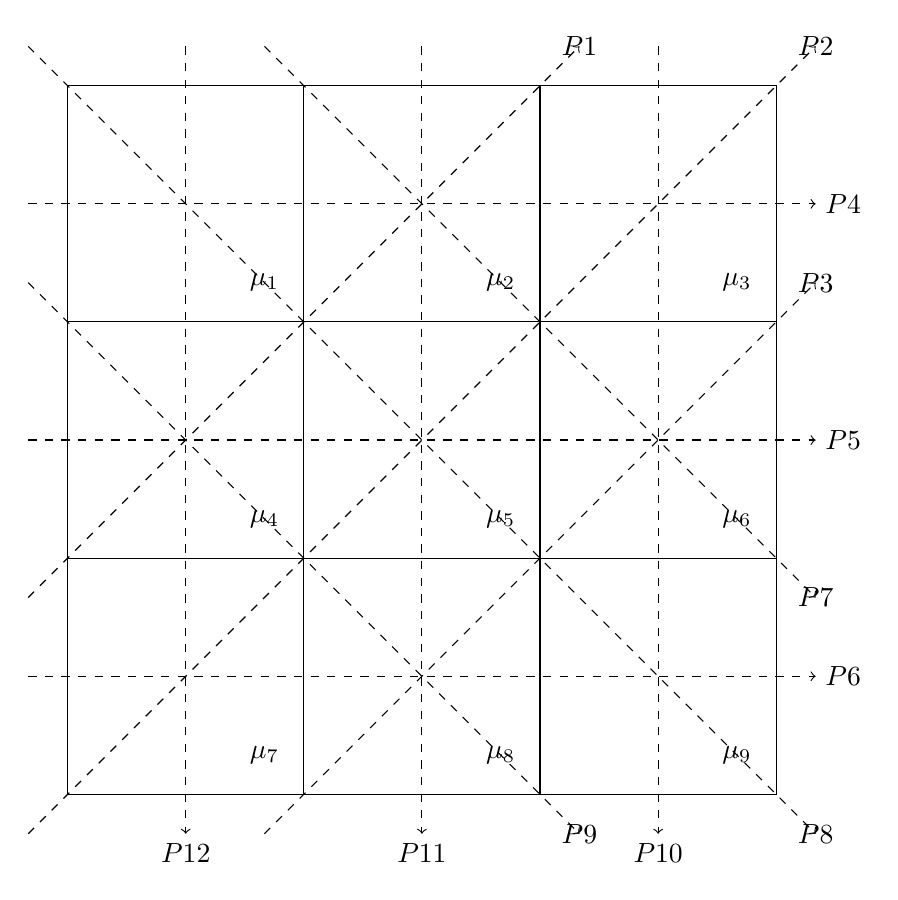
\begin{tikzpicture}
    \draw (0,9) -- (3,9) -- (3,6) -- (0,6) -- (0,9); % wuerfel 1
    \draw (3,9) -- (6,9) -- (6,6) -- (3,6) -- (3,9); % wuerfel 2
    \draw (6,9) -- (9,9) -- (9,6) -- (6,6) -- (6,9); % wuerfel 3
    \draw (0,6) -- (3,6) -- (3,3) -- (0,3) -- (0,6); % wuerfel 4
    \draw (3,6) -- (6,6) -- (6,3) -- (3,3) -- (3,6); % wuerfel 5
    \draw (6,6) -- (9,6) -- (9,3) -- (6,3) -- (6,6); % wuerfel 6
    \draw (0,3) -- (3,3) -- (3,0) -- (0,0) -- (0,3); % wuerfel 7
    \draw (3,3) -- (6,3) -- (6,0) -- (3,0) -- (3,3); % wuerfel 8
    \draw (6,3) -- (9,3) -- (9,0) -- (6,0) -- (6,3); % wuerfel 9
    \draw (2.5,6.5) node {$\symbf{\mu}_{1}$};
    \draw (5.5,6.5) node {$\symbf{\mu}_{2}$};
    \draw (8.5,6.5) node {$\symbf{\mu}_{3}$};
    \draw (2.5,3.5) node {$\symbf{\mu}_{4}$};
    \draw (5.5,3.5) node {$\symbf{\mu}_{5}$};
    \draw (8.5,3.5) node {$\symbf{\mu}_{6}$};
    \draw (2.5,0.5) node {$\symbf{\mu}_{7}$};
    \draw (5.5,0.5) node {$\symbf{\mu}_{8}$};
    \draw (8.5,0.5) node {$\symbf{\mu}_{9}$};
    % projektionsrichtungen
    \draw[->, dashed] (-0.5, 2.5) -- (6.5, 9.5) node {$P1$};
    \draw[->, dashed] (-0.5,-0.5) -- (9.5, 9.5) node {$P2$};
    \draw[->, dashed] (2.5, -0.5) -- (9.5, 6.5) node {$P3$};
    \draw[->, dashed] (-0.5, 7.5) -- (9.5, 7.5) node[right] {$P4$};
    \draw[->, dashed] (-0.5, 4.5) -- (9.5, 4.5) node[right] {$P5$};
    \draw[->, dashed] (-0.5, 1.5) -- (9.5, 1.5) node[right] {$P6$};
    \draw[->, dashed] ( 2.5, 9.5) -- (9.5, 2.5) node {$P7$};
    \draw[->, dashed] (-0.5, 9.5) -- (9.5,-0.5) node {$P8$};
    \draw[->, dashed] (-0.5, 6.5) -- (6.5,-0.5) node {$P9$};
    \draw[->, dashed] ( 1.5, 9.5) -- (1.5,-0.5) node[below] {$P12$};
    \draw[->, dashed] ( 4.5, 9.5) -- (4.5,-0.5) node[below] {$P11$};
    \draw[->, dashed] ( 7.5, 9.5) -- (7.5,-0.5) node[below] {$P10$};
  \end{tikzpicture}
  \caption{Abbildung der zwölf Projektionsrichtungen in einer Würfelebene mit je 9 kleineren Würfeln.}
  \label{fig:projection}
\end{figure}


\subsection{Absorptionsphänomene}
In diesem Versuch geht es um den Strahlungstyp Gammastrahlung, also Photonen.
Demnach gibt es drei Maßgebliche Wechselwirkungen,
welche bei der Absorption von Gammastrahlung auftreten können.
Zum einen der Photoeffekt, bei welchem die Photonen, wenn sie mindestens die Energie besitzen um ein Elektron zu ionisieren, eben dieses Elektron aus dem Material herausschlagen können.
Dann gibt es den \glname{Compton}{-Effekt},
bei welchem ein Photon an einem Elektron gestreut wird.
Das Photon hat nach der Streuung eine andere Wellenlänge als vorher.
Die Wellenlänge kann mit
\begin{equation}
  λ = \frac{\symup{c}}{ν} = \frac{\text{ch}}{E}
\end{equation}
in die Frequenz $ν$ und Energie $E$ umgeformt werden.
Zuletzt kann das noch zu Paarerzeugung kommen, wenn ein Photon mit mindestens der doppelten Elektronenmasse an Energie (d.h. 2x$\SI{511}{\kilo\electronvolt}$) in die Nähe eines Kerns gelangt.
Aufgrund der Energieerhaltung muss das Photon mindestens die doppelte Elektronenmasse als Energie besitzen.
Ein Kern wird als Stoßpartner gebraucht, da die Impulserhaltung gilt.

\subsection{Szintillationsdetektor}
Szintillationsdetektoren können sowohl aus organischen als auch anorganischen
Materialien bestehen. In diesem Fall haben wir einen anorganischen
Natriumiodidkristall verwendet.
Wenn ionisierende Strahlung mit einer bestimmten Energie größer als
die Anregungsenergie des Materials in dieses eindringt, springt ein
Elektron auf ein höheres Band und das Photon mit der Restenergie gestreut,
sodass es solange Atome ionisieren kann bis seine Energie nicht mehr
großgenug ist. 
Die so entstandenen Elektronen können nun mit den Löchern rekombinieren und
erzuegen dabei ein Photon mit der Energie der Bandlücke.
Die Photonen treten aus dem Szintillationsdetektor aus und gelangen in einen
Photomultiplier.
Dort wird an der Eingangskathode ein Elektron, durch den Photoeffekt, herausgelöst.
Dieses wird in einem System aus Elektroden beschleuigt und löst weitere Elektronen aus.
Dieser Strom kann dann detektiert werden und die Energie des Photons bestimmt werden. 
